\documentclass[12pt,a4paper]{article}
\usepackage[utf8]{inputenc}

\usepackage[a4paper]{geometry}

\usepackage{amsmath}
\usepackage{amsfonts}
\usepackage{amssymb}
\usepackage[english]{babel}
\usepackage{tikz}
%\usepackage{placeins}
\usepackage{graphicx}
%\usepackage{multirow}
%\usepackage{hyperref}

\setlength{\textwidth}{425px}
\setlength{\marginparwidth}{25px}

\makeatletter
\newcommand*{\rom}[1]{\expandafter\@slowromancap\romannumeral #1@}
\makeatother

\setlength{\parskip}{1ex plus 0.5ex minus 0.2ex}
\newcommand{\hsp}{\hspace{20pt}}
\newcommand{\HRule}{\rule{\linewidth}{0.5mm}}
\newenvironment{remarque}{\textbf{Remarque :}}{}



\title{Détails des cas d'utilisation de Paquito}
\author{PaquiTeam}


\begin{document}

\begin{titlepage}
	\begin{center}
	
		
		\vfill
					
		\textsc{\LARGE PaquiTeam}\\[1.5cm]
		
		% Title
		\HRule \\[0.4cm]
			{ \huge \bfseries Présentation des cas d'utilisation principaux :\\
			Paquito, easy packaging\\[0.4cm]
			
\includegraphics[width=0.2\textwidth]{../img/paquito.png}
	
			}
		\HRule \\[1.5cm]
		% Author and supervisor
		
		\begin{minipage}{0.40\textwidth}
			\begin{flushleft} \large
				\emph{Auteurs :}\\
				Lucas \textsc{Robin}\\
				Kevin \textsc{Fleuriot}\\
				Alexandre \textsc{Noiret}\\
				Yassine \textsc{Ait Elmouden}\\
				Seynabou \textsc{Ka}
			\end{flushleft}
		\end{minipage}
		\hfill
		\begin{minipage}{0.40\textwidth}
			\begin{flushright} \large
				\emph{Clients :}\\
				Michael \textsc{Fortier}\\
				Hugues \textsc{Leprieur}
			\end{flushright}
		\end{minipage}

		\vfill			
		{\large 21 janvier 2016}
		\vfill
		\begin{minipage}{0.35\textwidth}
			\begin{flushleft}
				
\includegraphics[width=1\textwidth]{../img/UP13.png}			
			\end{flushleft}
		\end{minipage}
		\hfill
		\begin{minipage}{0.35\textwidth}
			\begin{flushright}
				
\includegraphics[width=1\textwidth]{../img/sup-galile.png}
			\end{flushright}
		\end{minipage}
		
									
	\end{center}		
\end{titlepage}

\section*{Introduction}
Notre projet se porte sur l'outil Paquito, qui est un outil de génération de paquets pour un logiciel donné. Chaque paquet contient les fichiers de configuration nécessaires pour l'installation et l'utilisation du logiciel. Cet outil est utilisable pour plusieurs distributions de Linux. Le but de notre projet est donc d'améliorer l'utilisation de cet outil. Nous commencerons par transformer le programme en ligne de commande en un service web plus simple d'utilisation et plus complet qui permettra au développeur de rentrer toute ses informations dans un formulaire approprié ou en important directement un fichier YAML. Ensuite nous adapterons cet outil pour les distributions MacOS. 
	
Dans cet écrit nous allons vous exposer les différents cas d'utilisation de notre système ainsi qu'une première maquette de l'interface Web qui exploitera Paquito.

\section{Diagramme des cas d'utilisation}

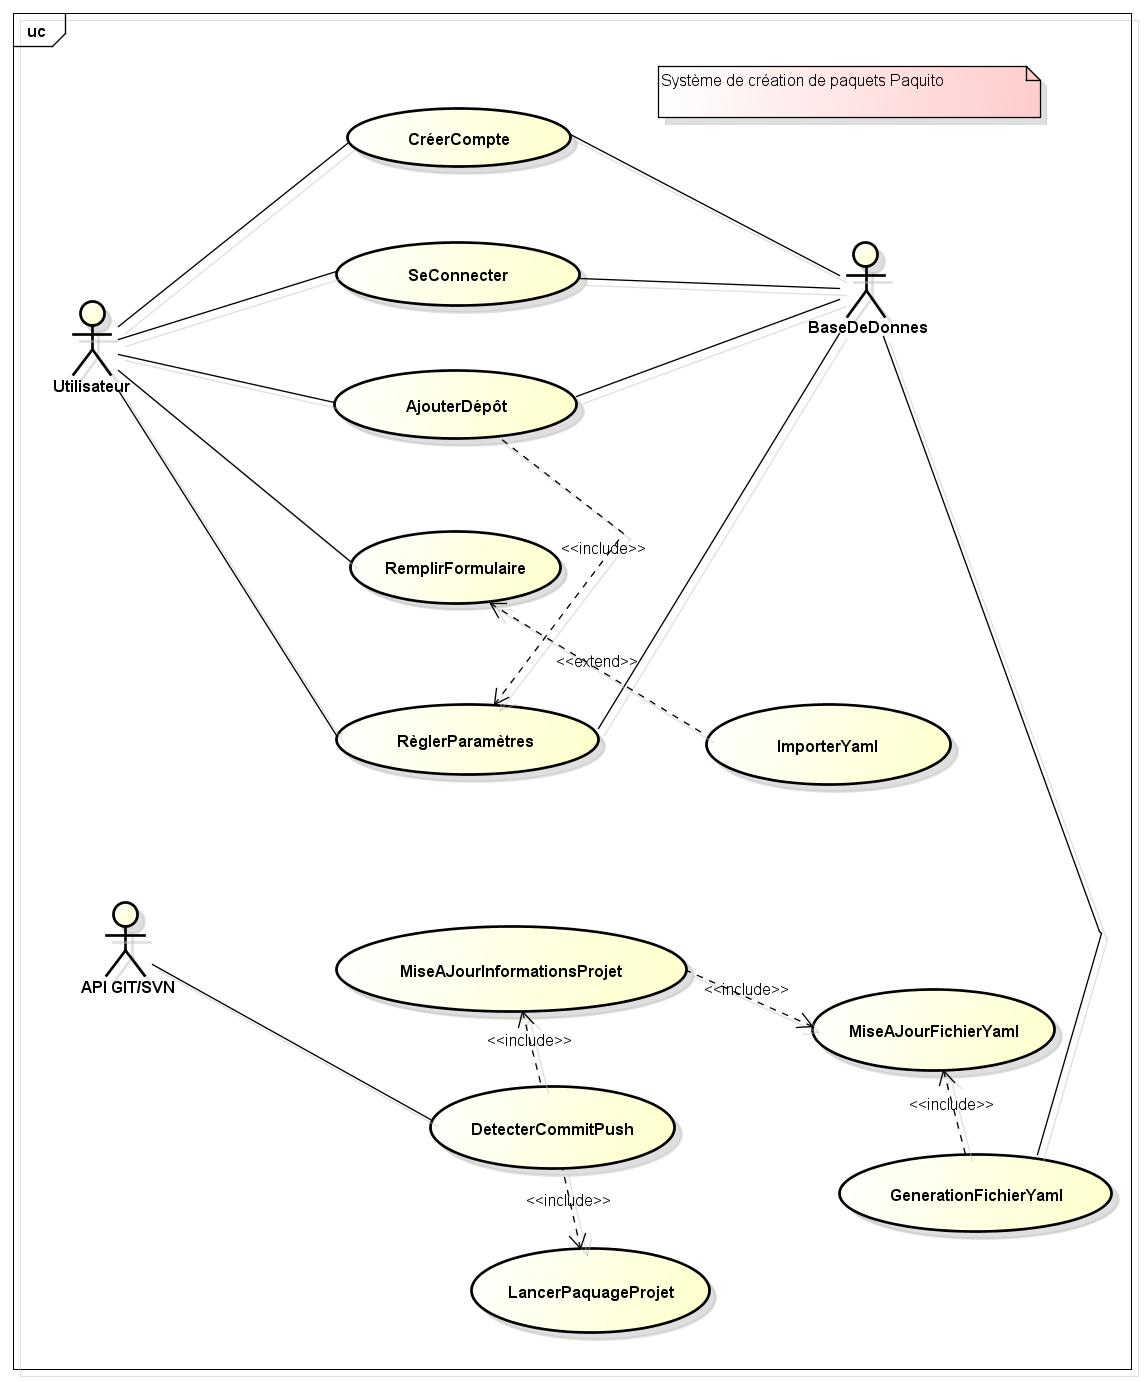
\includegraphics[scale=0.39]{../img/Diagram1_haut.jpg}

\section{Détails des cas d'utilisation}
\begin{itemize}\renewcommand{\labelitemi}{$\bullet$}
  
\item\textbf{\large Créer un compte} 
  \begin{itemize} 
  \item \textbf{Identification} 
    \begin{itemize} 
    \item[] Niveau de l'action : Sous-fonction 
    \item[] But : L'utilisateur (le développeur) crée un compte pour utiliser le service Web 
    \item[] Acteur : Utilisateur 
    \end{itemize} 
  \item \textbf{Scénario principal} 
    \begin{enumerate} 
    \item L'utilisateur renseigne ses coordonnées 
    \item Le site web accepte l'inscription 
    \end{enumerate}
  \end{itemize}
  
\item\textbf{\large Se connecter} 
  \begin{itemize} 
  \item \textbf{Identification} 
    \begin{itemize} 
    \item[] Niveau de l'action : Sous-fonction 
    \item[] But : L'utilisateur (le développeur) se connecte pour utiliser le service Web
    \item[] Acteur : Utilisateur 
    \end{itemize} 
  \item \textbf{Scénario principal} 
    \begin{enumerate} 
    \item L'utilisateur entre son login et son mot de passe 
    \item Le site web accepte l'inscription 
    \end{enumerate} 
  \item \textbf{Echec} 
    \begin{enumerate} 
    \item L'utilisateur n'est pas inscrit 
    \item Le site web notifie l'erreur et propose à l'utilisateur de s'inscrire 
    \item L'utilisateur est inscrit mais n'a pas renseigné le bon mot de passe 
    \item Le site web notifie l'erreur et propose à l'utilisateur de recommencer 
    \end{enumerate} 
  \end{itemize}
  
\item\textbf{\large Ajouter un dépôt} 
  \begin{itemize} 
  \item \textbf{Identification} 
    \begin{itemize} 
    \item[] Niveau de l'action : But utilisateur 
    \item[] But : L'utilisateur ajoute un dépôt sur le service Web pour un projet.
    \item[] Acteur : Utilisateur 
    \end{itemize} 
  \item \textbf{Scénario principal} 
    \begin{enumerate}
    \item L'utilisateur indique le nom et l'URL du dépôt. 
    \item Le serveur est contacté et lance la commande d'ajout de dépôt. 
    \end{enumerate} 
  \end{itemize}
  
\item\textbf{\large Mise à jour des informations du projet}
  \begin{itemize}
  \item \textbf{Identification}
    \begin{itemize}
    \item[] Niveau de l'action : Sous fonction
    \item[] But : Mettre à jour les informations du projet
    \item[] Acteur : Utilisateur
    \end{itemize}
  \item \textbf{Scénario principal}
    \begin{enumerate}
    \item L'utilisateur change les informations via l'application web
    \item Les informations sont changées suite à un commit ou un push
    \item Changement des informations dans la Base de Donnée
    \item Génération du nouveau fichier YAML
    \end{enumerate}
  \end{itemize}
  
\item \textbf{Gérer paramètres de création de paquets} : On peut modifier les paramètres de création des paquets
  
\item\textbf{\large Lancement du paquetage du projet}
  \begin{itemize}
  \item \textbf{Identification}
    \begin{itemize}
    \item[] Niveau de l'action : Sous fonction
    \item[] But : Créer les fichiers qui composent le paquetage et genère le fichier contenant les informations sur le paquetage
    \item[] Acteur : API GIT/SVN
    \end{itemize}
  \item \textbf{Scénario principal}
    \begin{enumerate}
    \item Les sources et le fichier YAML ainsi que d'autres informations sont envoyées, via ssh par exemple, aux Machines Virtuelles.
    \item Lancement de l'opération de compilation.
    \item On notifie le(s) développeur(s) de la réussite de la création du paquetage
    \end{enumerate}
  \item \textbf{Echec}
    \begin{itemize}
    \item En cas d'erreur lors de la création du paquetage on envoie une notification au(x) développeur(s) avec l'erreur retournée par Paquito
    \end{itemize}
  \end{itemize}
  
\item\textbf{\large Détection de Commit ou de Push}
  \begin{itemize}
  \item \textbf{Identification}
    \begin{itemize}
    \item[] Niveau de l'action : Sous fonction
    \item[] But : L’API GIT/SVN détecte un changement, qui est notamment un commit ou un push.
    \item[] Acteur : API GIT/ SVN
    \end{itemize}
  \item \textbf{Scénario principal}
    \begin{enumerate}
    \item Un développeur fait un commit/push sur son dépôt.
    \item Le serveur en est averti via l’API Git/Svn
    \item Les informations du projet ont été mises à jour
    \item Lancement de la compilation et paquetage sur les Machines Virtuelles du projet.
    \end{enumerate}
  \end{itemize}

\item\textbf{\large Remplir formulaire}
  \begin{itemize}
  \item \textbf{Identification}
    \begin{itemize}
    \item[] Niveau de l'action : Sous fonction
    \item[] But : L'utilisateur rempli les informations sur le projet qu'il veut faire suivre par paquito
    \item[] Acteur : Utilisateur
    \end{itemize}
  \item \textbf{Scénario principal}
    \begin{enumerate}
    \item L'utilisateur rempli tous les champs
    \item L'utilisateur soumet le formulaire
    \end{enumerate}
  \item \textbf{Echec}
    \begin{itemize}
    \item Un ou plusieurs champs ne sont pas remplis
    \end{itemize}
  \end{itemize}

\item\textbf{\large Importer un fichier YAML}
  \begin{itemize}
  \item \textbf{Identification}
    \begin{itemize}
    \item[] Niveau de l'action : Sous-fonction
    \item[] But : Importer un fichier YAML lorsque l'utilisateur l'a déjà en sa disposition
    \item[] Acteur : Utilisateur
    \end{itemize}
  \item \textbf{Scénario principal}
    \begin{enumerate}
    \item L'utilisateur va envoyer son fichier YAML via l'application Web
    \item Le système va lire le fichier et remplir automatiquement le formulaire sur l'application Web.
    \end{enumerate}
  \end{itemize}
  
  
%\item\textbf{\large }
%  \begin{itemize}
%  \item \textbf{Identification}
%    \begin{itemize}
%    \item[] Niveau de l'action :
%    \item[] But :
%    \item[] Acteur :
%    \end{itemize}
%  \item \textbf{Scénario principal}
%    \begin{enumerate}
%    \item 
%    \end{enumerate}
%  \end{itemize}
  
\end{itemize}

\section{Base de données}
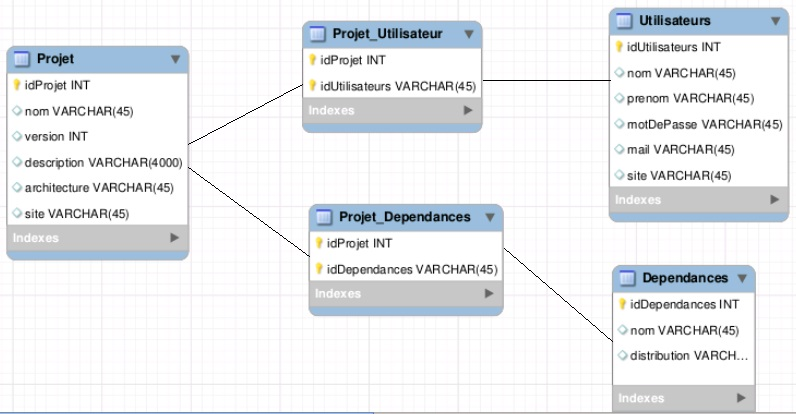
\includegraphics[scale=0.8]{../img/bdd.jpg}

\section{Maquette du site}
	Nous avons aussi fait des maquettes de l'interface graphique afin de pouvoir visualiser a quoi elle devra ressembler.

Nous avons dans un premier temps, la maquette de la page de connexion, cela reste classique avec un login et un mot de passe pour s'inscrire et se connecter.
	
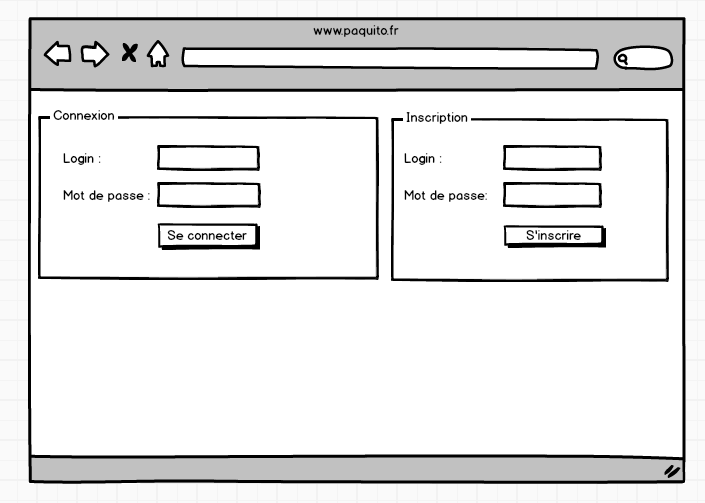
\includegraphics[scale=0.7]{../img/connexionPaquito.png}

Nous avons ensuite l'interface d'ajout de projet à Paquito où il y a un onglet à remplir pour que par la suite Paquito puisse compiler et créer les paquets en fonction de la distribution si une personne voudrait l'installer sur sa machine.

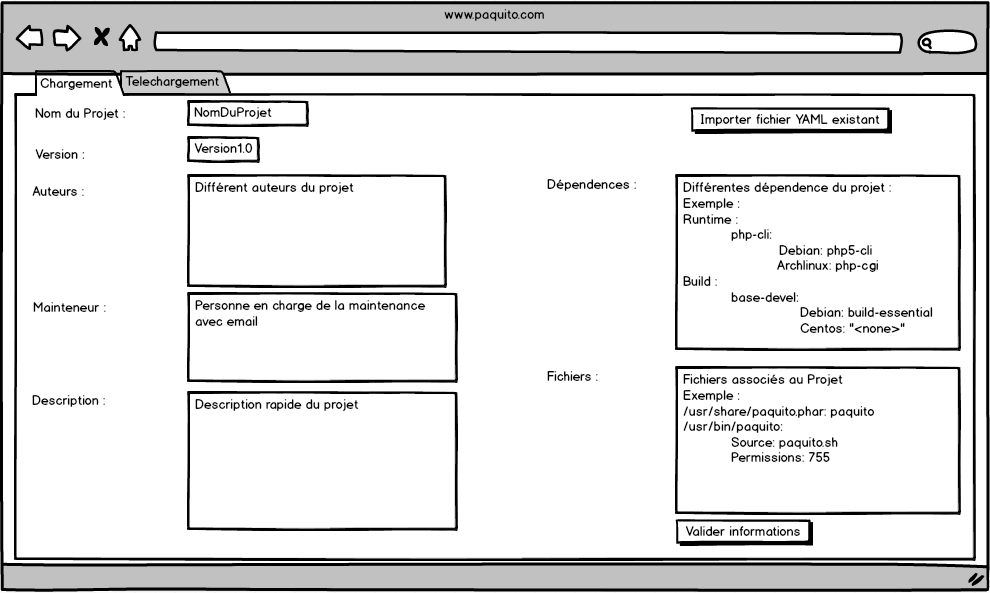
\includegraphics[scale=0.5]{../img/ajouterProjet.png}

Puis nous avons la vue d'une page où l'on peut voir des détails sur le projet comme le nom du développeur, le nom du projet.

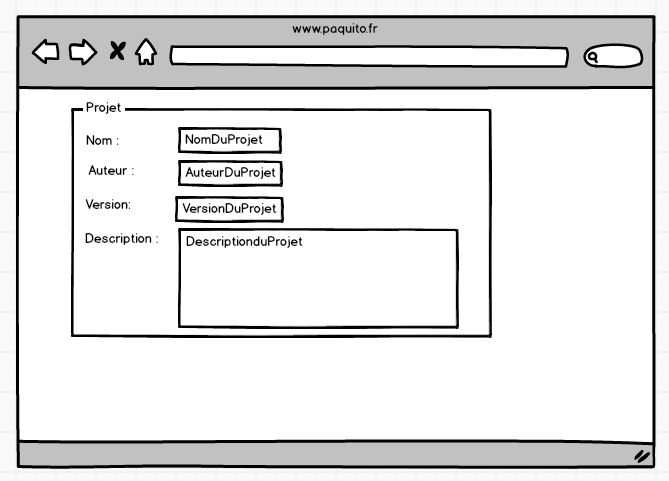
\includegraphics[scale=0.6]{../img/resumeProjet.png}

Et enfin, la page pour télécharger les paquets générés.

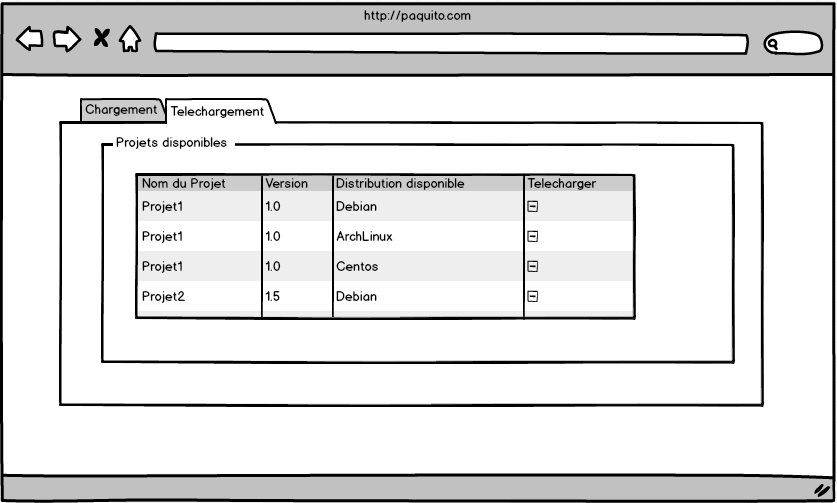
\includegraphics[scale=0.6]{../img/telechargerProjet.png}
	
\end{document}
